\chapter{Google Form : validation du projet}
\label{annexe:googleForm}

\section{Choix de vos rôles}

\begin{figure}[H]
    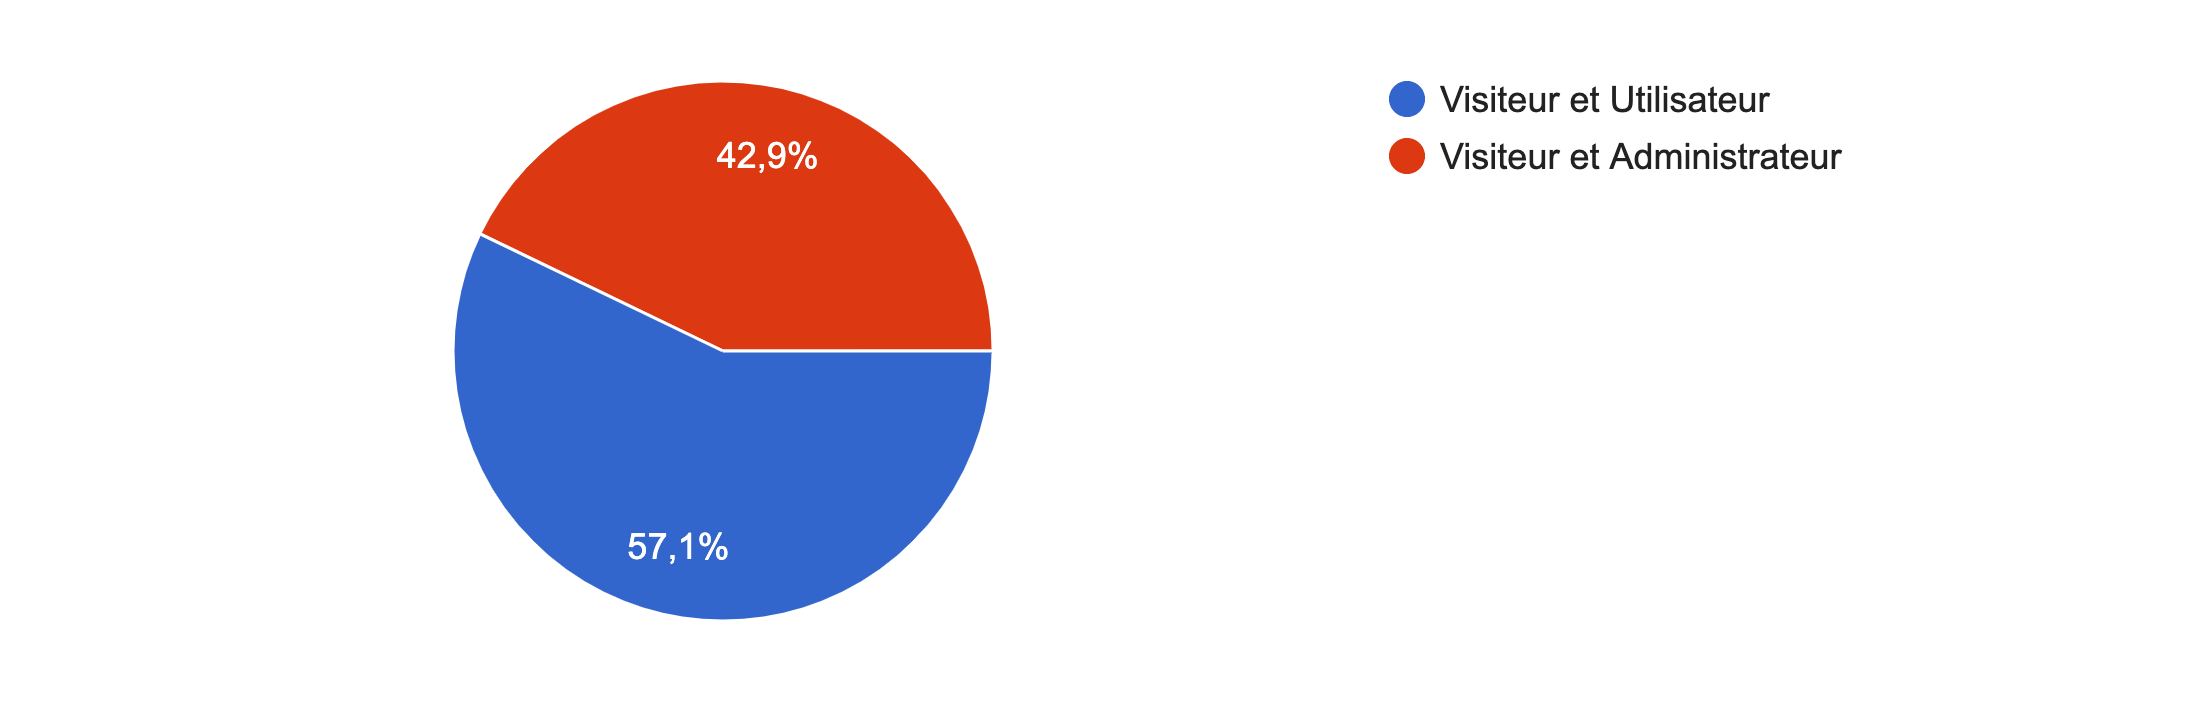
\includegraphics[width=\textwidth,height=0.3\textheight,keepaspectratio]{images/googleForm/roles.png}
    \centering
\end{figure}

\section{Rôles : Visiteur et utilisateur}

\subsection{Premier rôle : Visiteur}

\subsubsection*{Des remarques sur votre expérience avec ce rôle ?}

\begin{itemize}
    \item Système intuitif, clair et très riche en filtres, permettant de cibler/retrouver rapidement l'exo potentiellement recherché.\\
    Petite remarque, mais pas importante et peut-être personnelle: la "barre de recherche" laisse penser qu'il s'agit d'une recherche à travers tout le site et non pas directement au sein de la bibliothèque (peut-être parce qu'elle est placée dans le header et non pas au sein de la "page" bibliothèque ?)
    \item Simple et intuitif
    \item La barre de recherche textuelle est placée en haut du site, comme si c'était pour rechercher sur le domaine entier. Je pense qu'elle serait mieux mise un peu plus bas, à droite de "réinitialiser ma recherche" par exemple.
\end{itemize}

\subsection{Deuxième rôle : Utilisateur}

\subsubsection*{Des remarques sur votre expérience avec ce rôle ?}

\begin{itemize}
    \item Pas de remarque
\end{itemize}

\subsection{Questionnaire}


\subsubsection*{Esthétique \& Ergonomie}

\begin{figure}[H]
    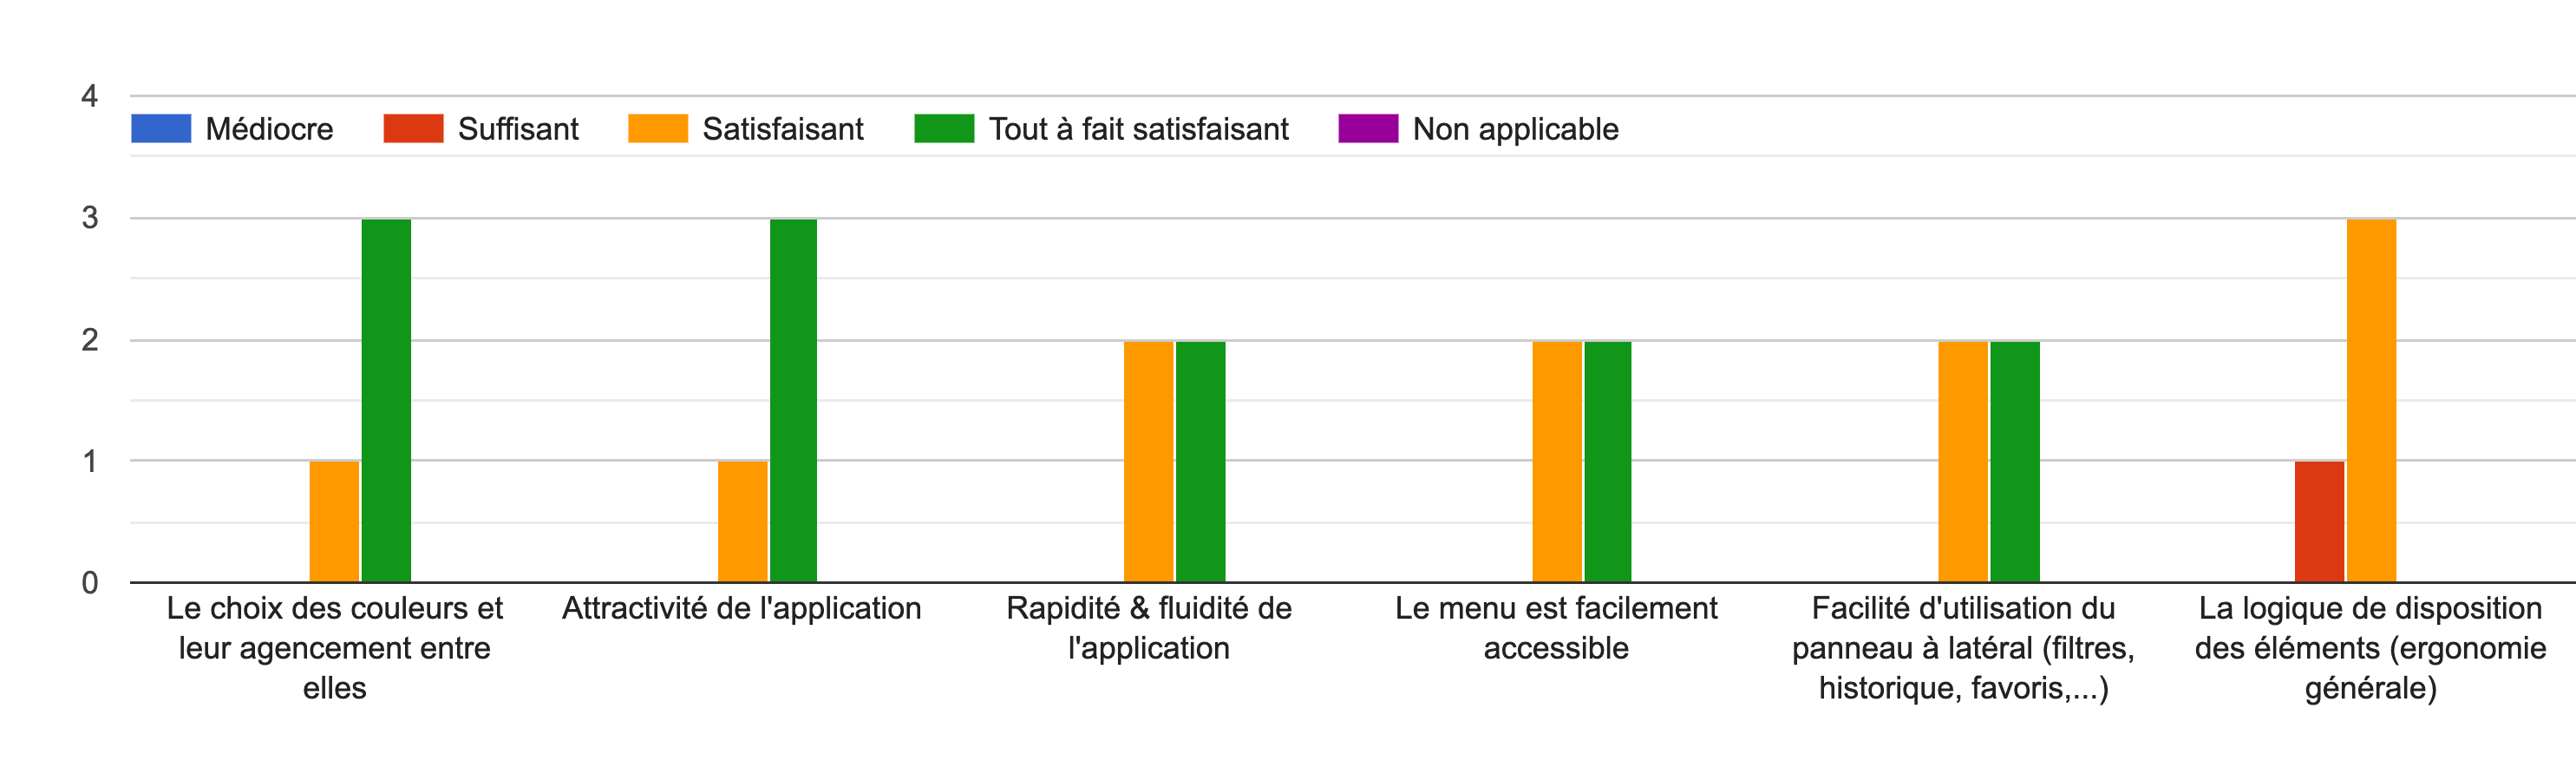
\includegraphics[width=\textwidth,height=0.3\textheight,keepaspectratio]{images/googleForm/ergonomie_1.png}
    \centering
\end{figure}


\subsubsection*{Des remarques ?}

\begin{itemize}
    \item ++ Très chouette ! Remarque similaire à la précédente, avec la barre de recherche dans le header.\\
    Je dois avouer que le bouton "retour" dans le header est également un peu perturbant, je ne l'ai découvert qu'après un petit moment d'utilisation du site. Son emplacement est peut-être moins intuitif.
    \item peut etre la barre de recherche pour les exercices et les chevrons dans le menu de gauche pas nécessaires
    \item Je pense tout a été dit dans l'appel :)
    \item Un dark mode ? Personnaliser le thème de couleurs ?
\end{itemize}


\subsubsection*{Page bibliothèque}

\begin{figure}[H]
    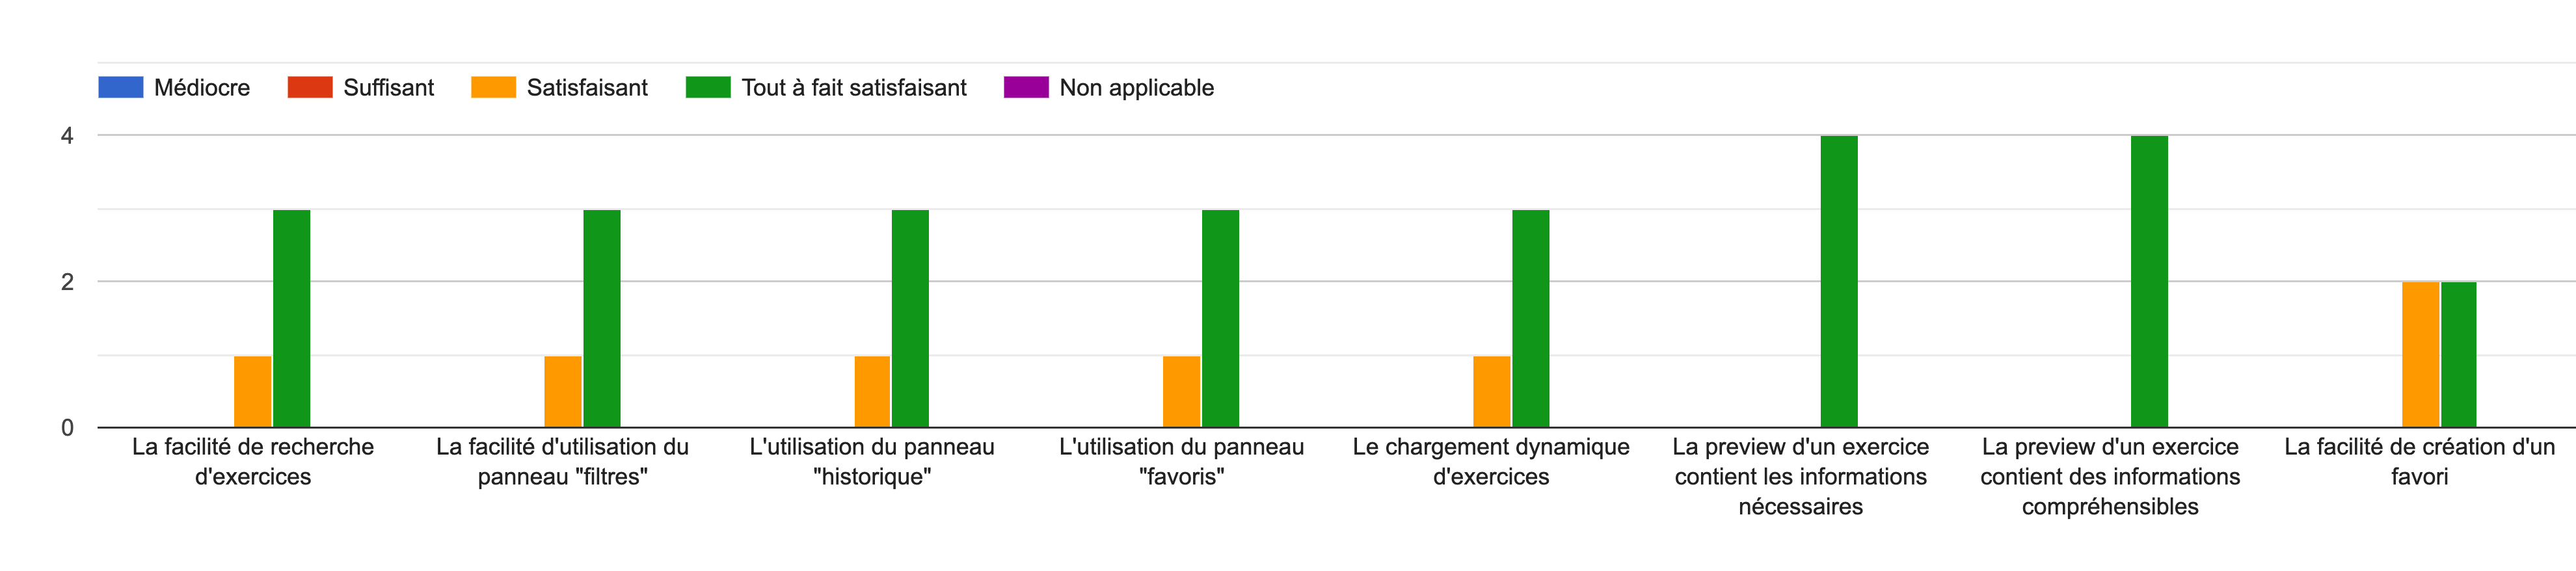
\includegraphics[width=\textwidth,height=0.3\textheight,keepaspectratio]{images/googleForm/bibliotheque_1.png}
    \centering
\end{figure}

\subsubsection*{Des remarques ?}

\begin{itemize}
    \item Vraiment un détails mais à la création d'un favori, si une fois le nom entré, la touche "enter" permettait de directement créer le favori au lieu de devoir cliquer, ça pourrait être sympa (mais de nouveau, on est dans le détails)
    \item Petites remarques:
    \begin{itemize}
        \item Si je suis dans la bibliothèque, que je clique sur l'onglet Favoris et que je choisis d'en modifier un, (j'arrive donc sur la page de modification du favori) le bouton de retour (dans le header) me propose de retourner dans "Mes favoris", alors que je venais de la bibliothèque.
        \item Toujours en étant dans l'onglet Favoris de la Bibliothèque, si je clique sur le "stylet" me permettant d'aller modifier le favori, ça exécute le favori (ça lance la recherche) avant de me transférer à la page de modification du favori.
    \end{itemize} 
    \item Juste je pense pas nécessaire d'avoir un tag pour créer un favori
\end{itemize}

\subsubsection*{Page d'une ressource informatique}

\begin{figure}[H]
    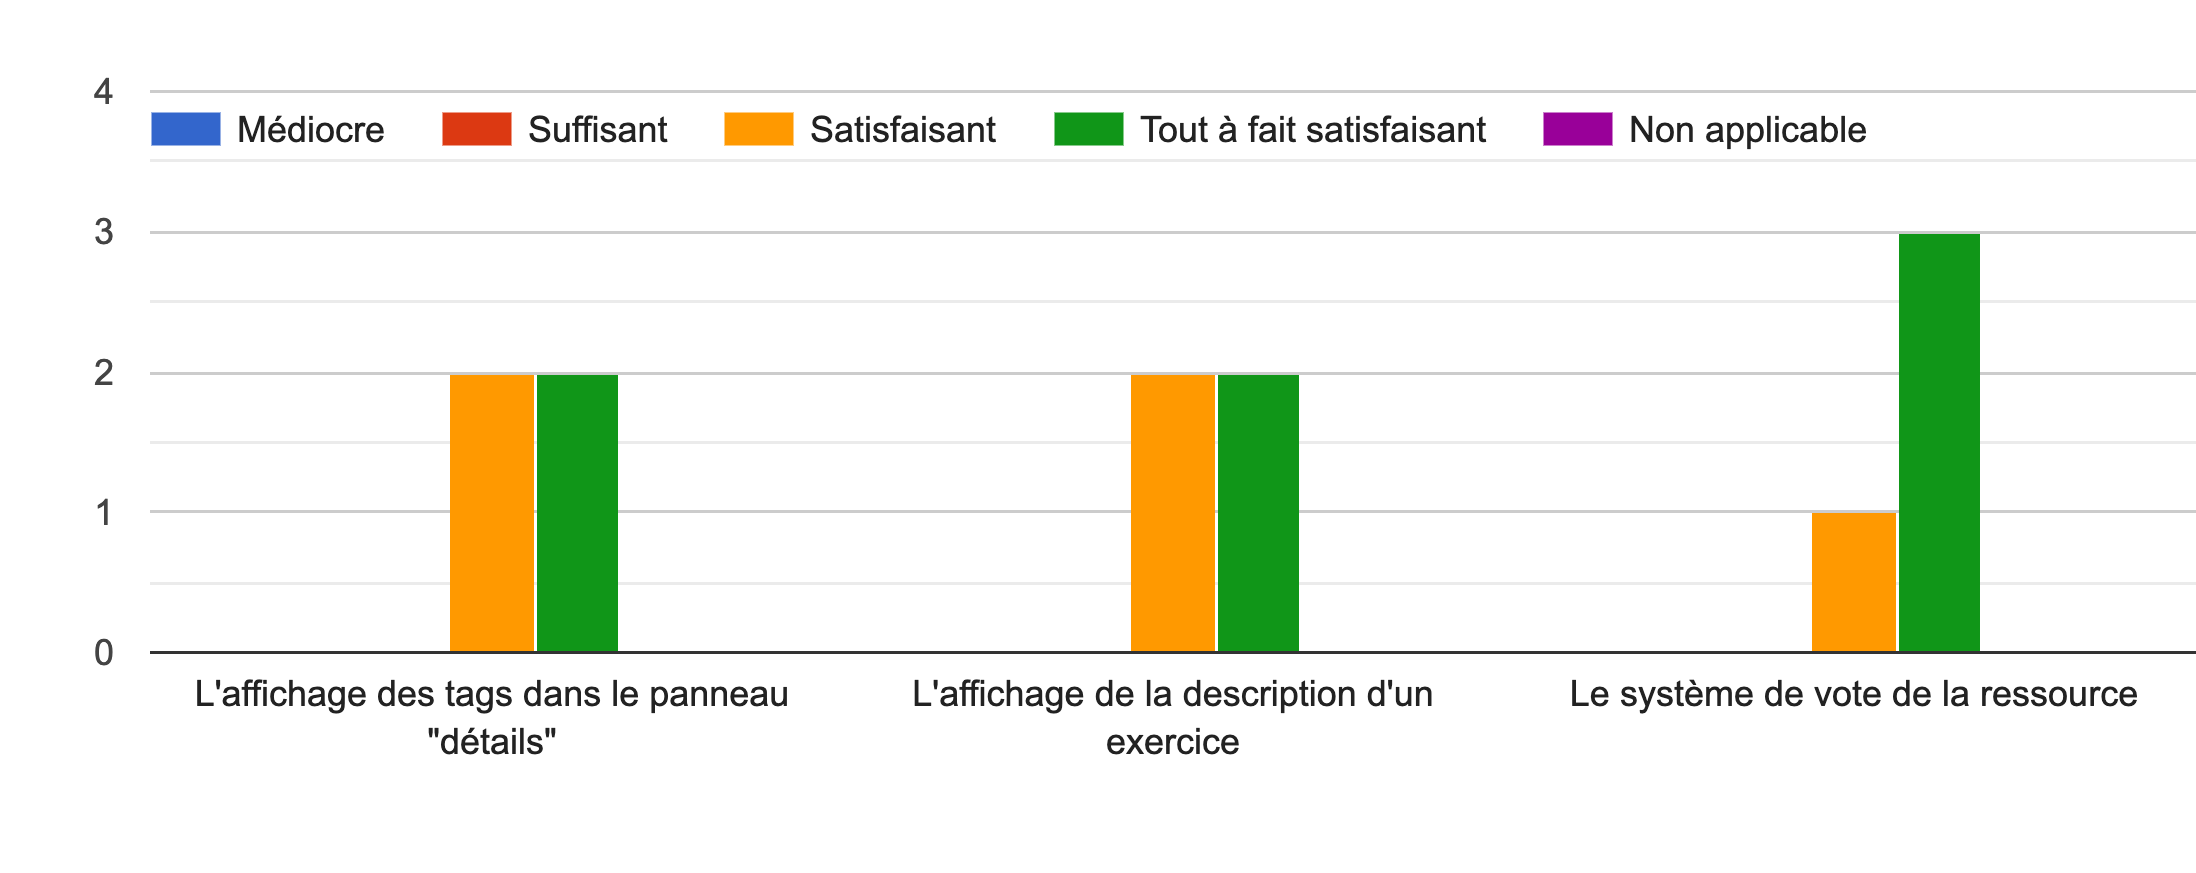
\includegraphics[width=\textwidth,height=0.3\textheight,keepaspectratio]{images/googleForm/resinfo_1.png}
    \centering
\end{figure}

\subsubsection*{Des remarques ?}

\begin{itemize}
    \item Il n'y a actuellement aucune réponse à cette question.
\end{itemize}

\subsubsection*{Page des favoris}

\begin{figure}[H]
    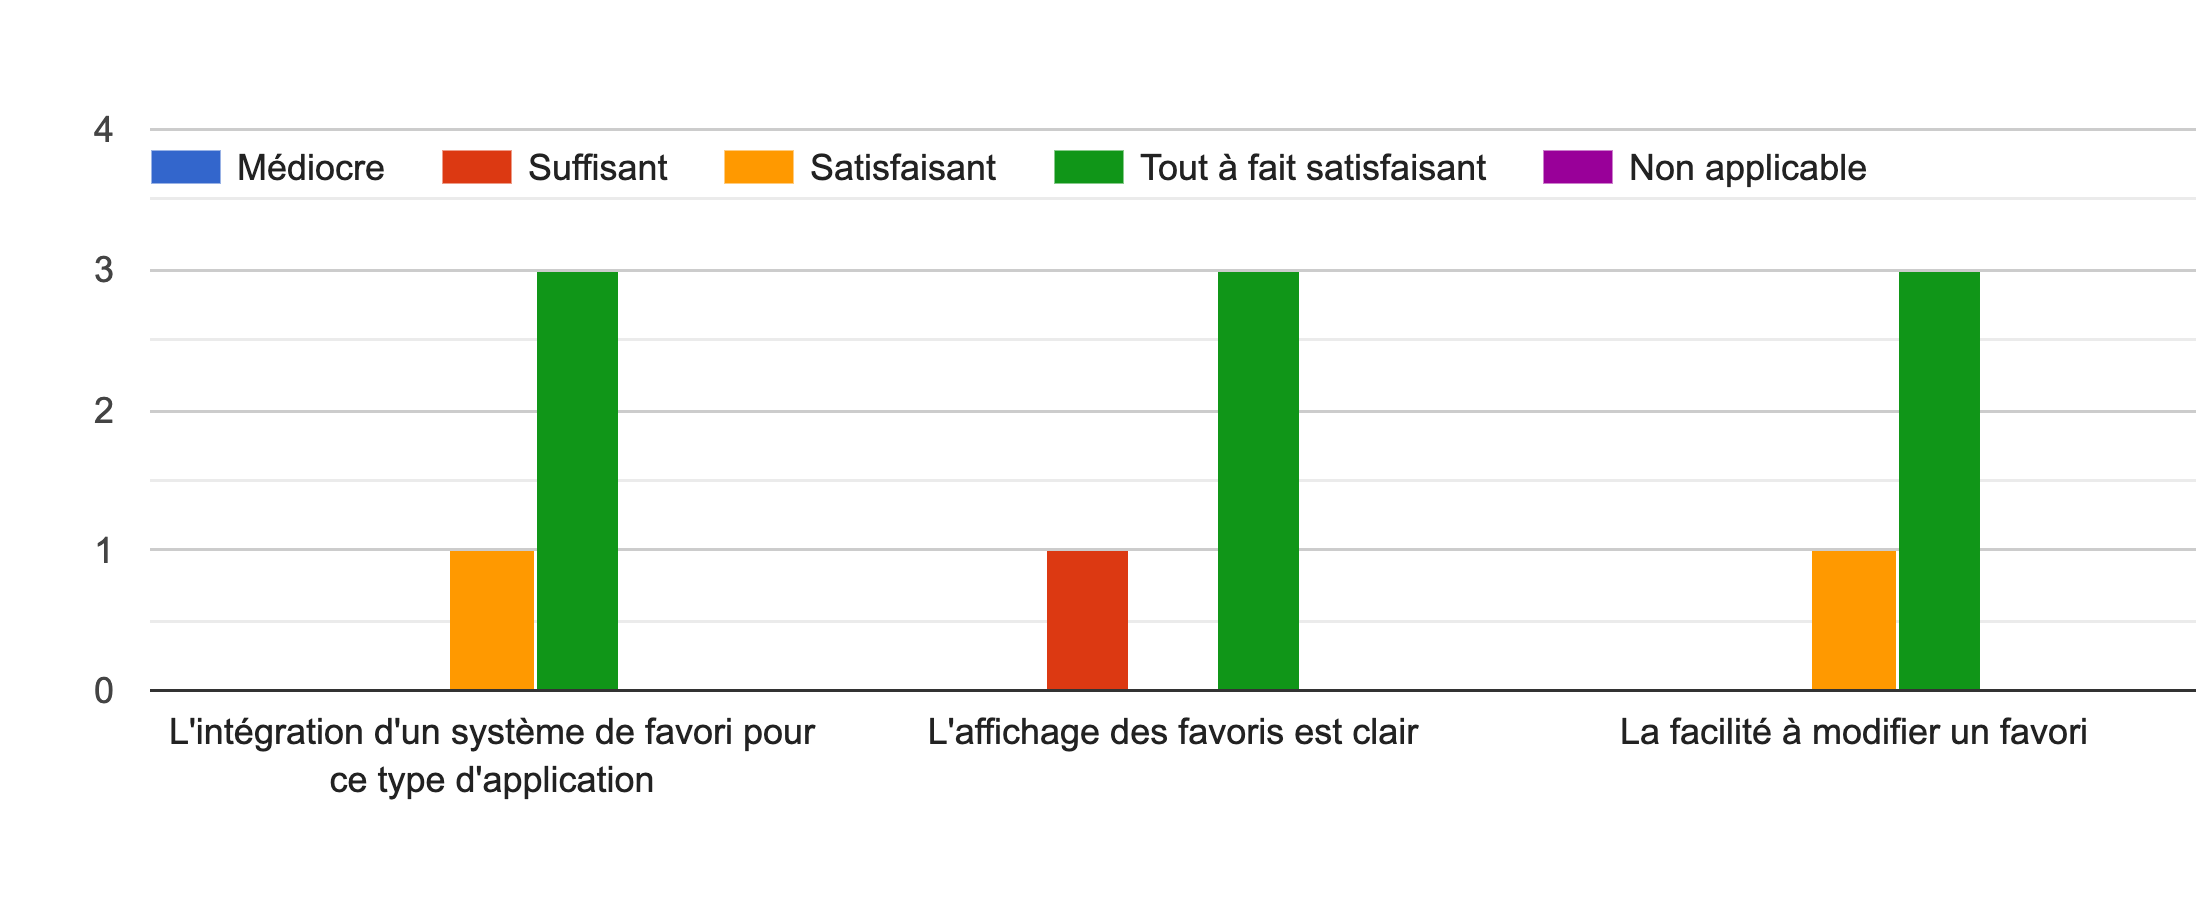
\includegraphics[width=\textwidth,height=0.3\textheight,keepaspectratio]{images/googleForm/favoris_1.png}
    \centering
\end{figure}

\subsubsection*{Des remarques ?}

\begin{itemize}
    \item Petit détails mais, je crée un favori en sélectionnant plusieurs tags de plusieurs catégories. Parmi eux, je choisis "non spécifié" (Langage). Je reviens par la suite pour modifier mon favori, je revois donc ma liste de tags choisis et je vois "non spécifié", sauf que.. Difficile de se souvenir de quelle catégorie il s'agit. Peut-être renommer des tags pas assez parlant, ou alors lorsque l'on est sur la page de modification du favori et que l'on clique sur un des tags déjà présents, ça ouvre le menu déroulant des tags au bon endroit (nous permettant de directement savoir de quelle catégorie il s'agit)
    \item Manque d'informations dans les carte favoris de la bibilothèques, on ne devrait pas avoir à retourner dans la liste de fav pour voir ce que fait le favoris
\end{itemize}


\subsubsection*{Page de gestion des ressources informatiques}

\begin{figure}[H]
    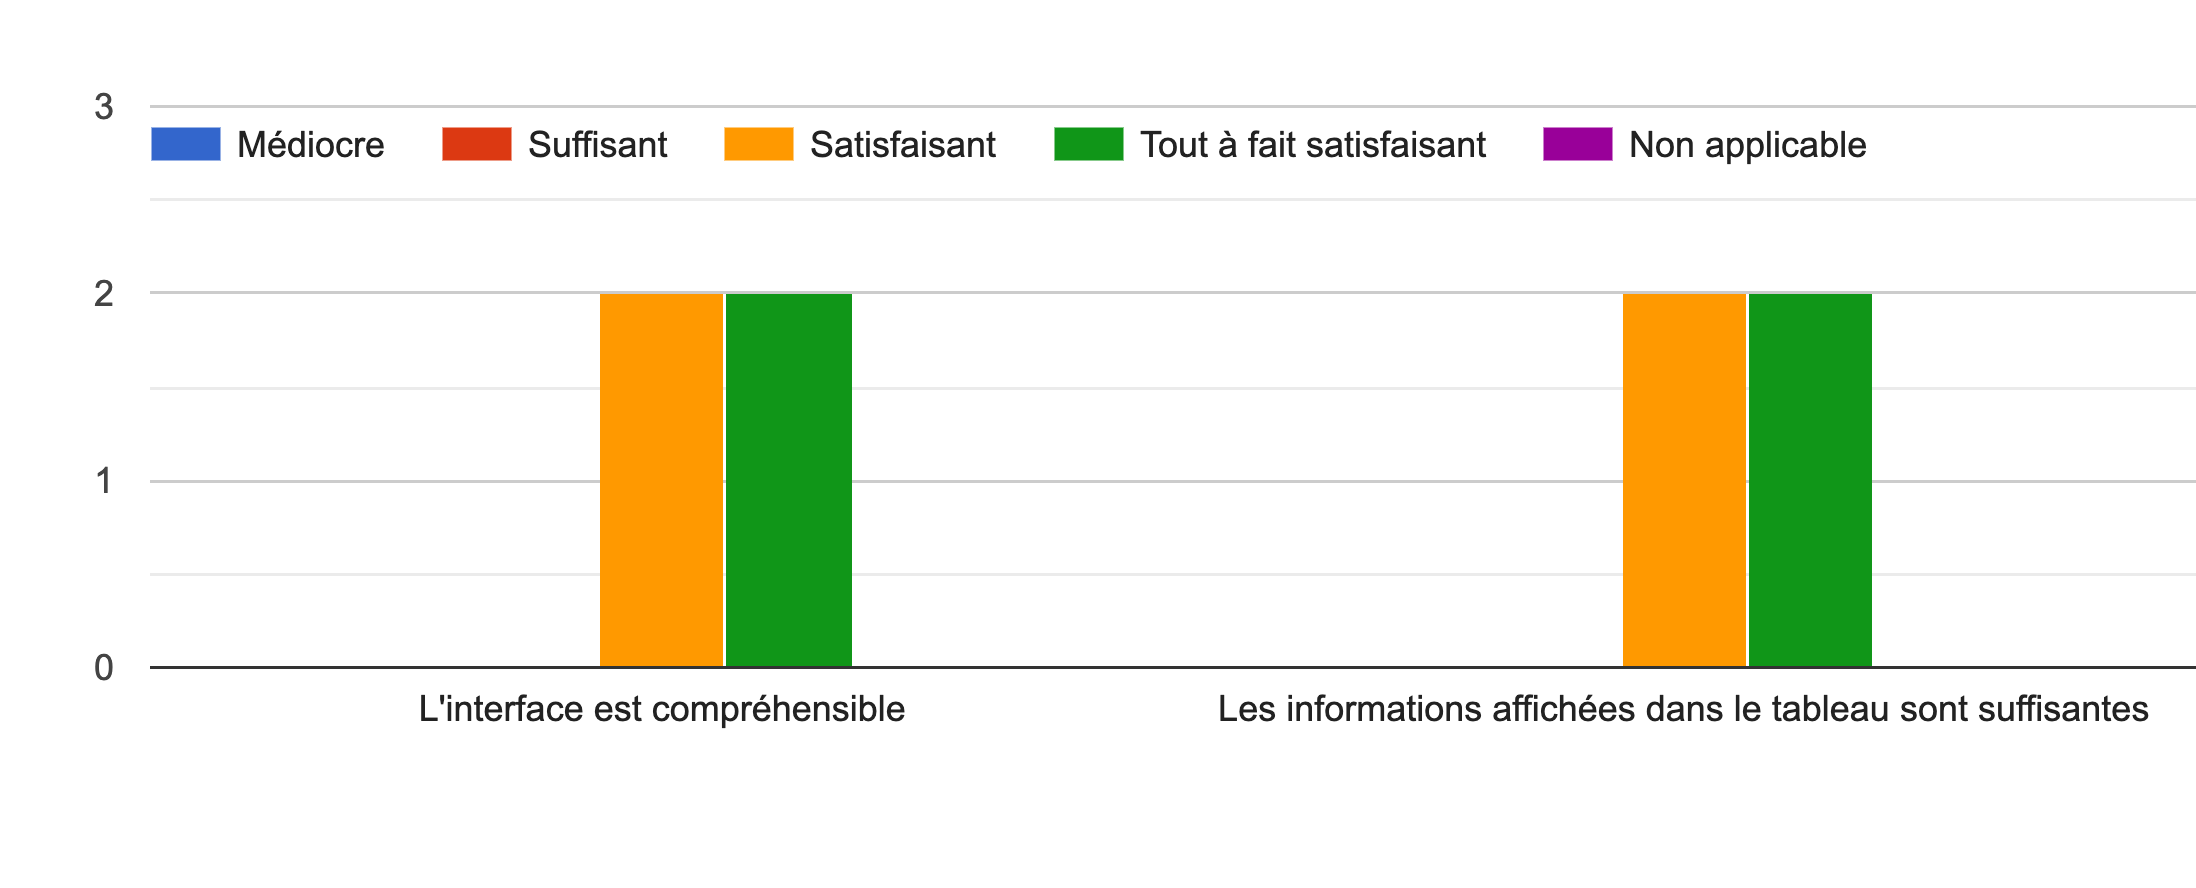
\includegraphics[width=\textwidth,height=0.3\textheight,keepaspectratio]{images/googleForm/gestionResInfo_1.png}
    \centering
\end{figure}

\subsubsection*{Des remarques ?}

\begin{itemize}
    \item Il n'y a actuellement aucune réponse à cette question.
\end{itemize}

\subsubsection*{Page de création/modification d'une ressource informatique}

\begin{figure}[H]
    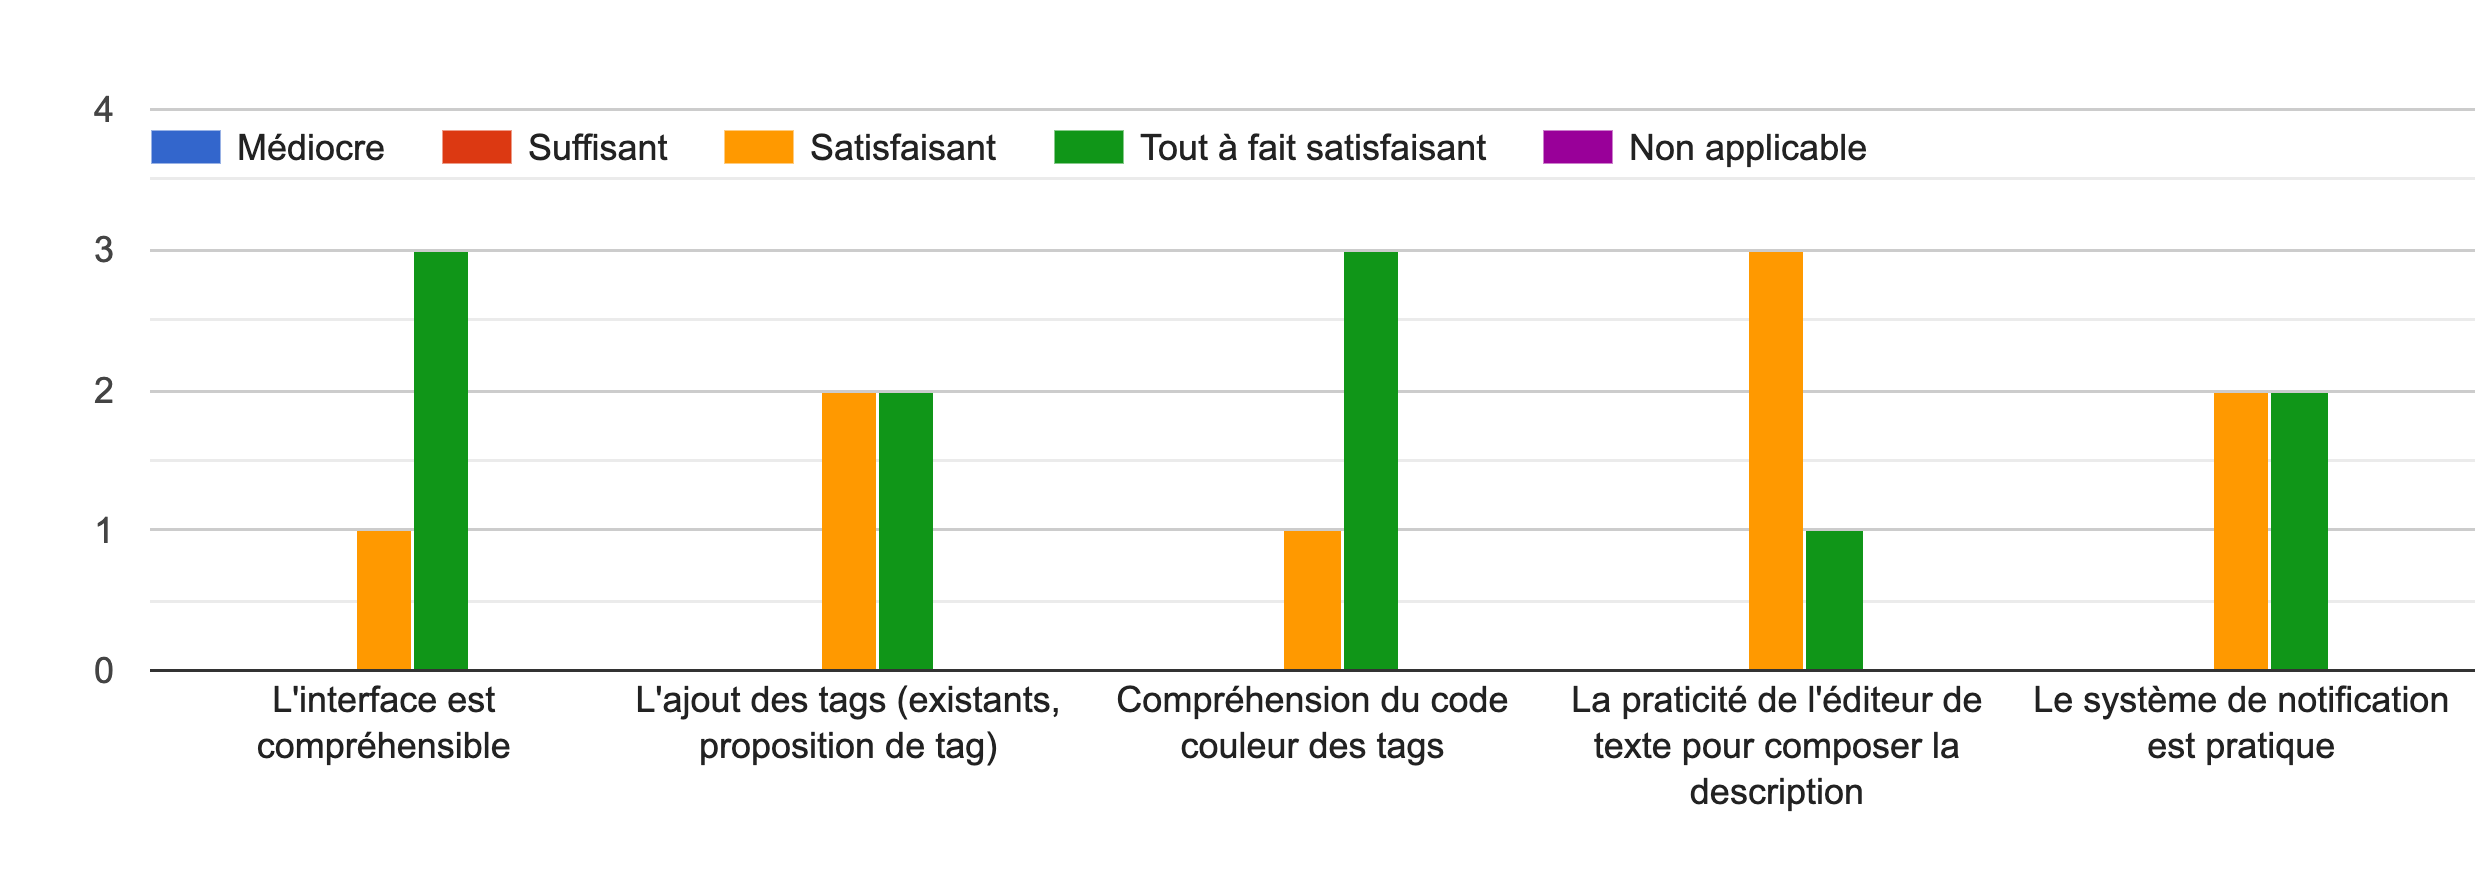
\includegraphics[width=\textwidth,height=0.3\textheight,keepaspectratio]{images/googleForm/creationModifResInfo_1.png}
    \centering
\end{figure}

\subsubsection*{Des remarques ?}

\begin{itemize}
    \item (((Interligne peut-être un peu grande)))\\
    Frustrant de pas pouvoir créer un bloc de code directement depuis plusieurs lignes sélectionnées. (Peut-être ne pas trop miser sur la page 'Tutoriel', je suis pas certain que les gens ont tendance à se rendre sur des manuels pour comprendre un outils)
    \item Glitch UI : quand on est sur "mes exercices" et qu'on clique sur "créer un exercice" les exercices disparaissent.
\end{itemize}

\section{Visiteur et Administrateur (modérateur)}

\subsection{Premier rôle : Visiteur}

\subsubsection*{Des remarques sur votre expérience avec ce rôle ?}

\begin{itemize}
    \item Quelques remarques :
    \begin{itemize}
        \item proposition: Gestion des fautes de frappes et/ou de la recherche approximative.
        \item Le texte de la barre de recherche est trop petit, et en bleu trop clair.
        \item La barre de recherche d'exercices est dans la barre principale, et donne l'impression qu'elle recherche dans tout le site. Elle est trop loin des filtres.
        \item Cf. image de github pour avoir des catégories de tags (i.e. filtres)
    \end{itemize}
    \item Plutôt fluide. Eu un peu de mal à scroller dans les listes de tags par filtres (Cliquer sur "languages" puis scroll jusqu'à Java). Il y a bien deux scroll bars mais ce n'est pas super intuitif
    \item Tout s'est bien passé. 2 petites remarques d'ergonomie : la double liste déroulante dans le panneau des tags lorsqu'une catégorie est sélectionnée m'a un peu perturbée. Et je n'ai pas trouvé tout de suite dans la barre de recherche (action 2)
\end{itemize}


\subsection{Deuxième rôle : Administrateur}

\subsubsection*{Des remarques sur votre expérience avec ce rôle ?}

\begin{itemize}
    \item Editeur de texte !!!!
    \begin{itemize}
        \item Pas de <tab>
        \item Sélectionner plusieurs lignes pour en faire un bloc de code génère un bloc de code par ligne.
        \item Possibilité d'agrandir la boite de texte si besoin (handle)
        \item Petit bug avec le copier-coller et les fins de ligne (unix/windows)
    \end{itemize}
    Les tags représentés par un filtre, sur le côté, c'est louche. Pas fait le 5 de admin.
    \item J'ai malencontreusement supprimer le tag admin en attente sans faire exprès et n'ai pas pu tester ça, mais à part l'absence de possibilité d'indenter mon code dans l'éditeur, ça va. Encore une fois, le tab des tags est un peu difficile à utiliser, mais dès la seconde utilisation ça passe/
    \item Pas de souci majeur rencontré dans le cadre de cette expérience.
\end{itemize}


\subsection{Questionnaire}

\subsubsection*{Esthétique \& Ergonomie}

\begin{figure}[H]
    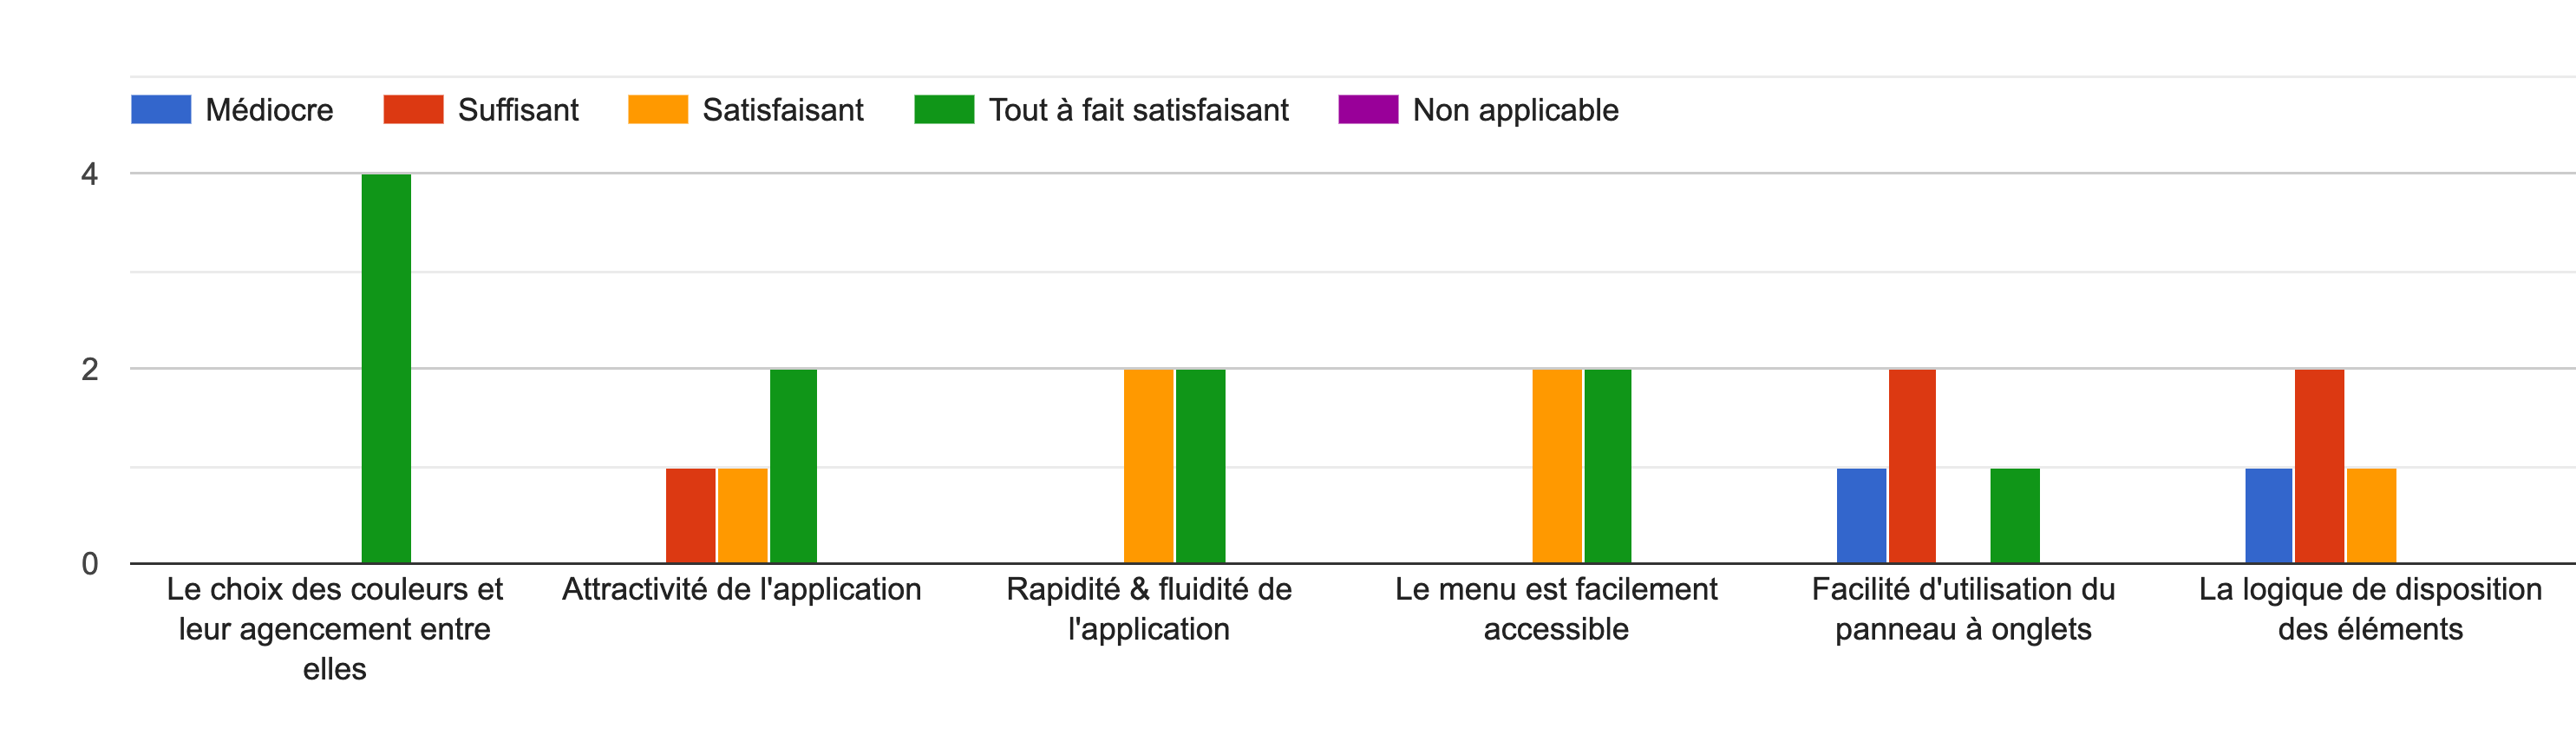
\includegraphics[width=\textwidth,height=0.3\textheight,keepaspectratio]{images/googleForm/ergonomie_2.png}
    \centering
\end{figure}

\subsubsection*{Des remarques ?}

\begin{itemize}
    \item Bien joué !
    \item Tout a été dit dans l'appel je pense :)
    \item On en a parlé, mais le menu filtres/tags est un peu trop détaché de ce qu'on est en train de faire
    \item Attention à la zone de recherche de la page bibliothèque qui semble décalée de tout le reste. De plus, les 2 icônes s'y trouvant semblent beaucoup plus petites que le reste de la page.
\end{itemize}


\subsubsection*{Bibliothèque}

\begin{figure}[H]
    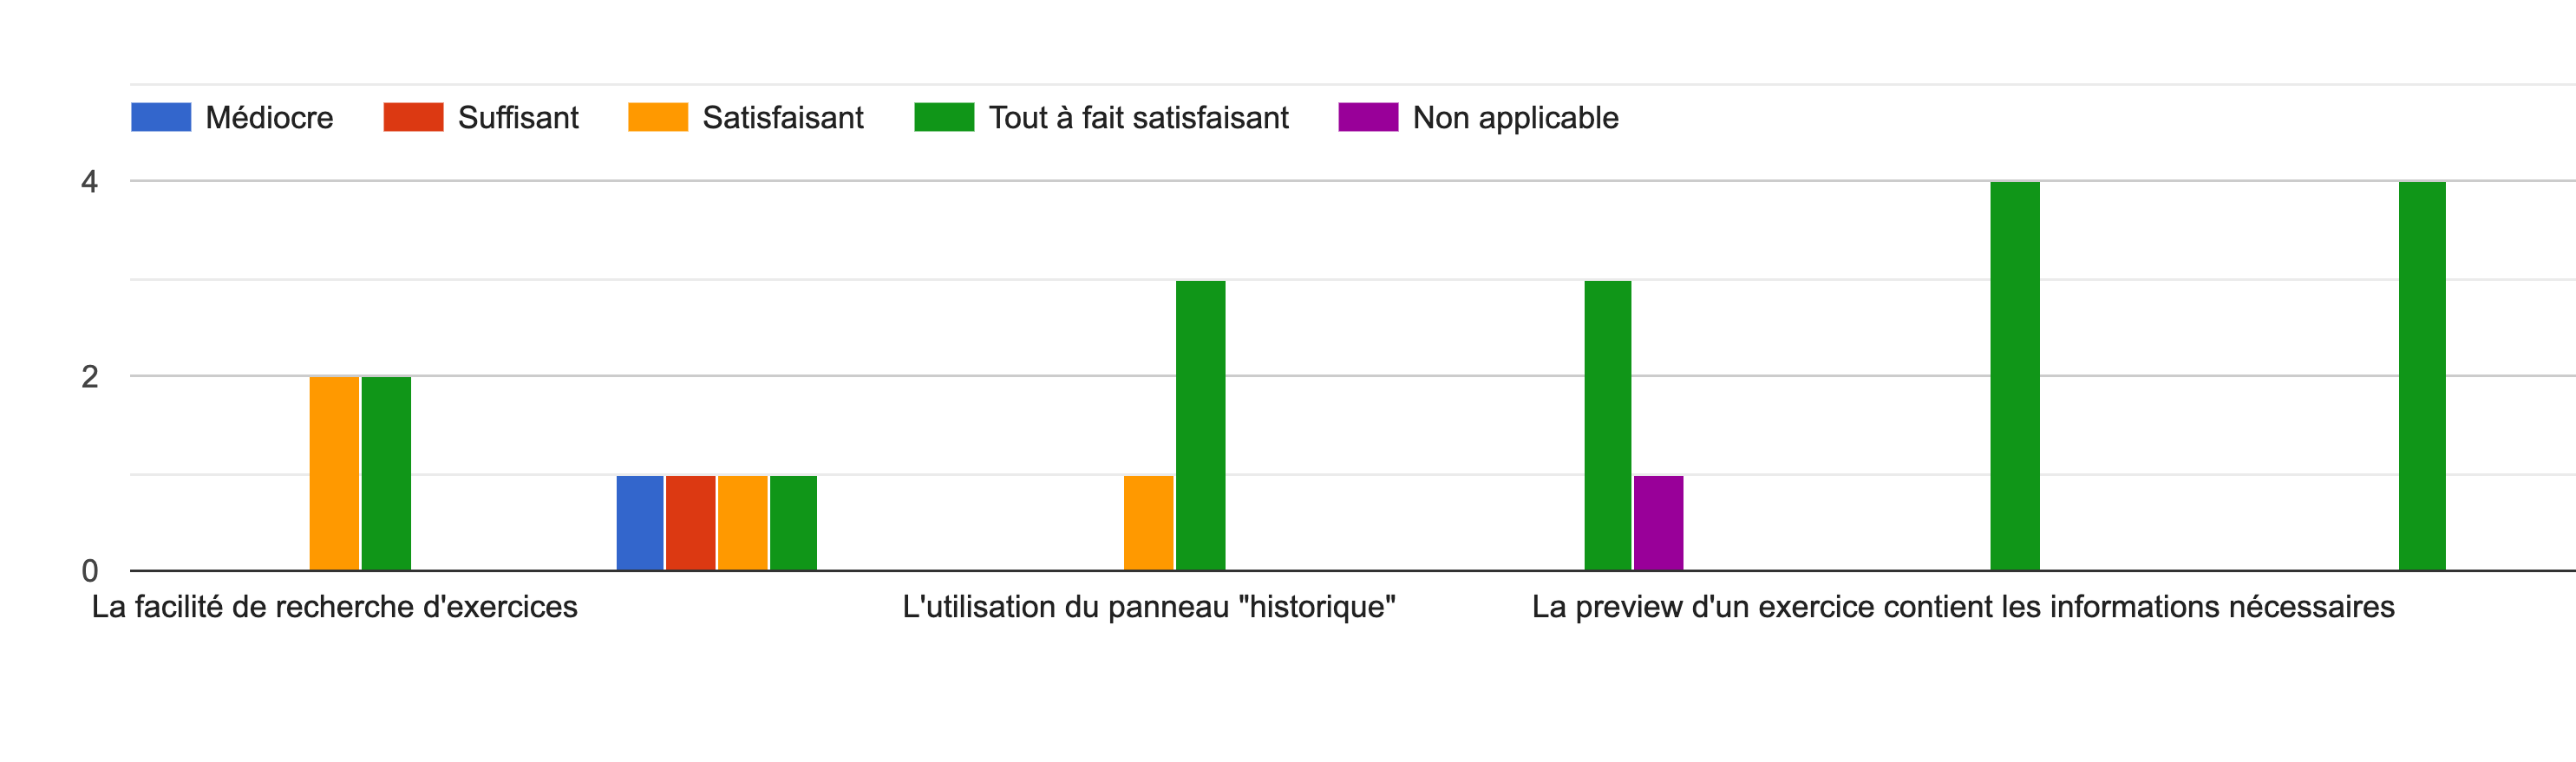
\includegraphics[width=\textwidth,height=0.3\textheight,keepaspectratio]{images/googleForm/bibliotheque_2.png}
    \centering
\end{figure}

\subsubsection*{Des remarques ?}

\begin{itemize}
    \item Il n'y a actuellement aucune réponse à cette question.
\end{itemize}


\subsubsection*{Page d'une ressource informatique}

\begin{figure}[H]
    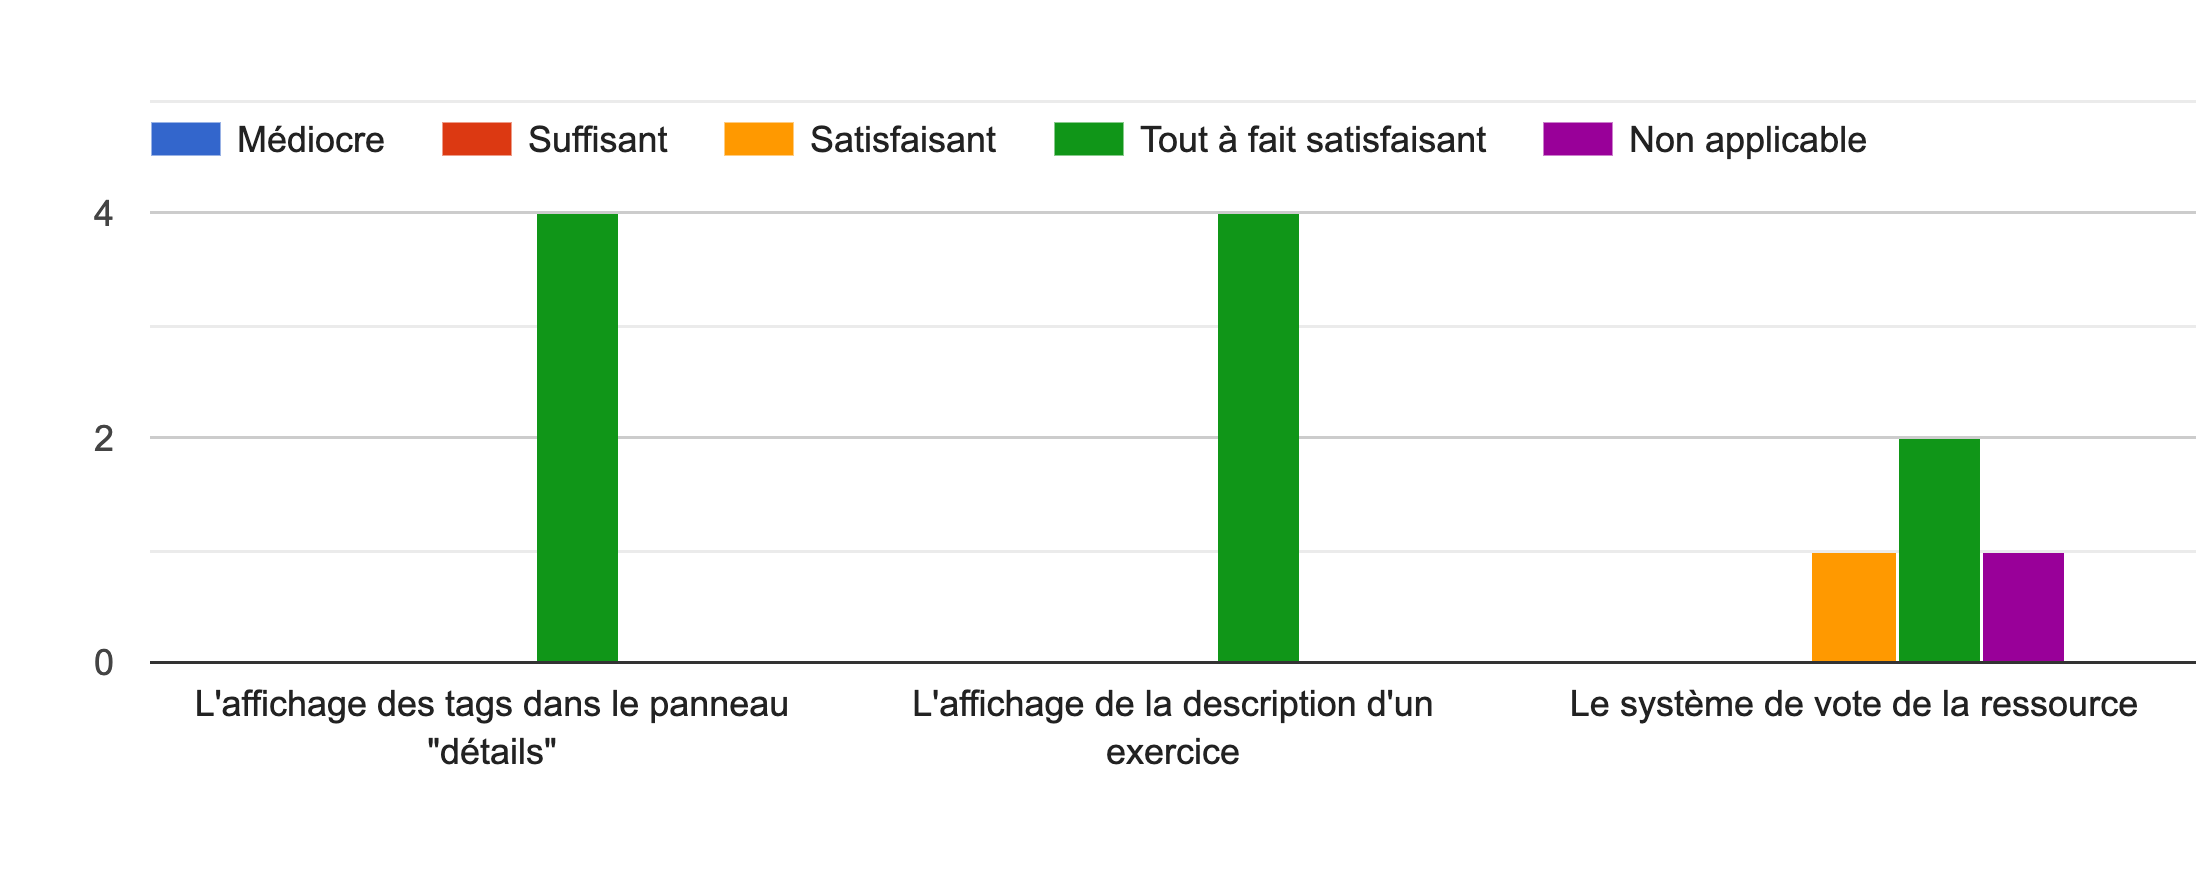
\includegraphics[width=\textwidth,height=0.3\textheight,keepaspectratio]{images/googleForm/resinfo_2.png}
    \centering
\end{figure}

\subsubsection*{Des remarques ?}

\begin{itemize}
    \item C'est beau ! Ca me semble être la page la plus accomplie ;)
\end{itemize}


\subsubsection*{Page de gestion des ressources informatiques}

\begin{figure}[H]
    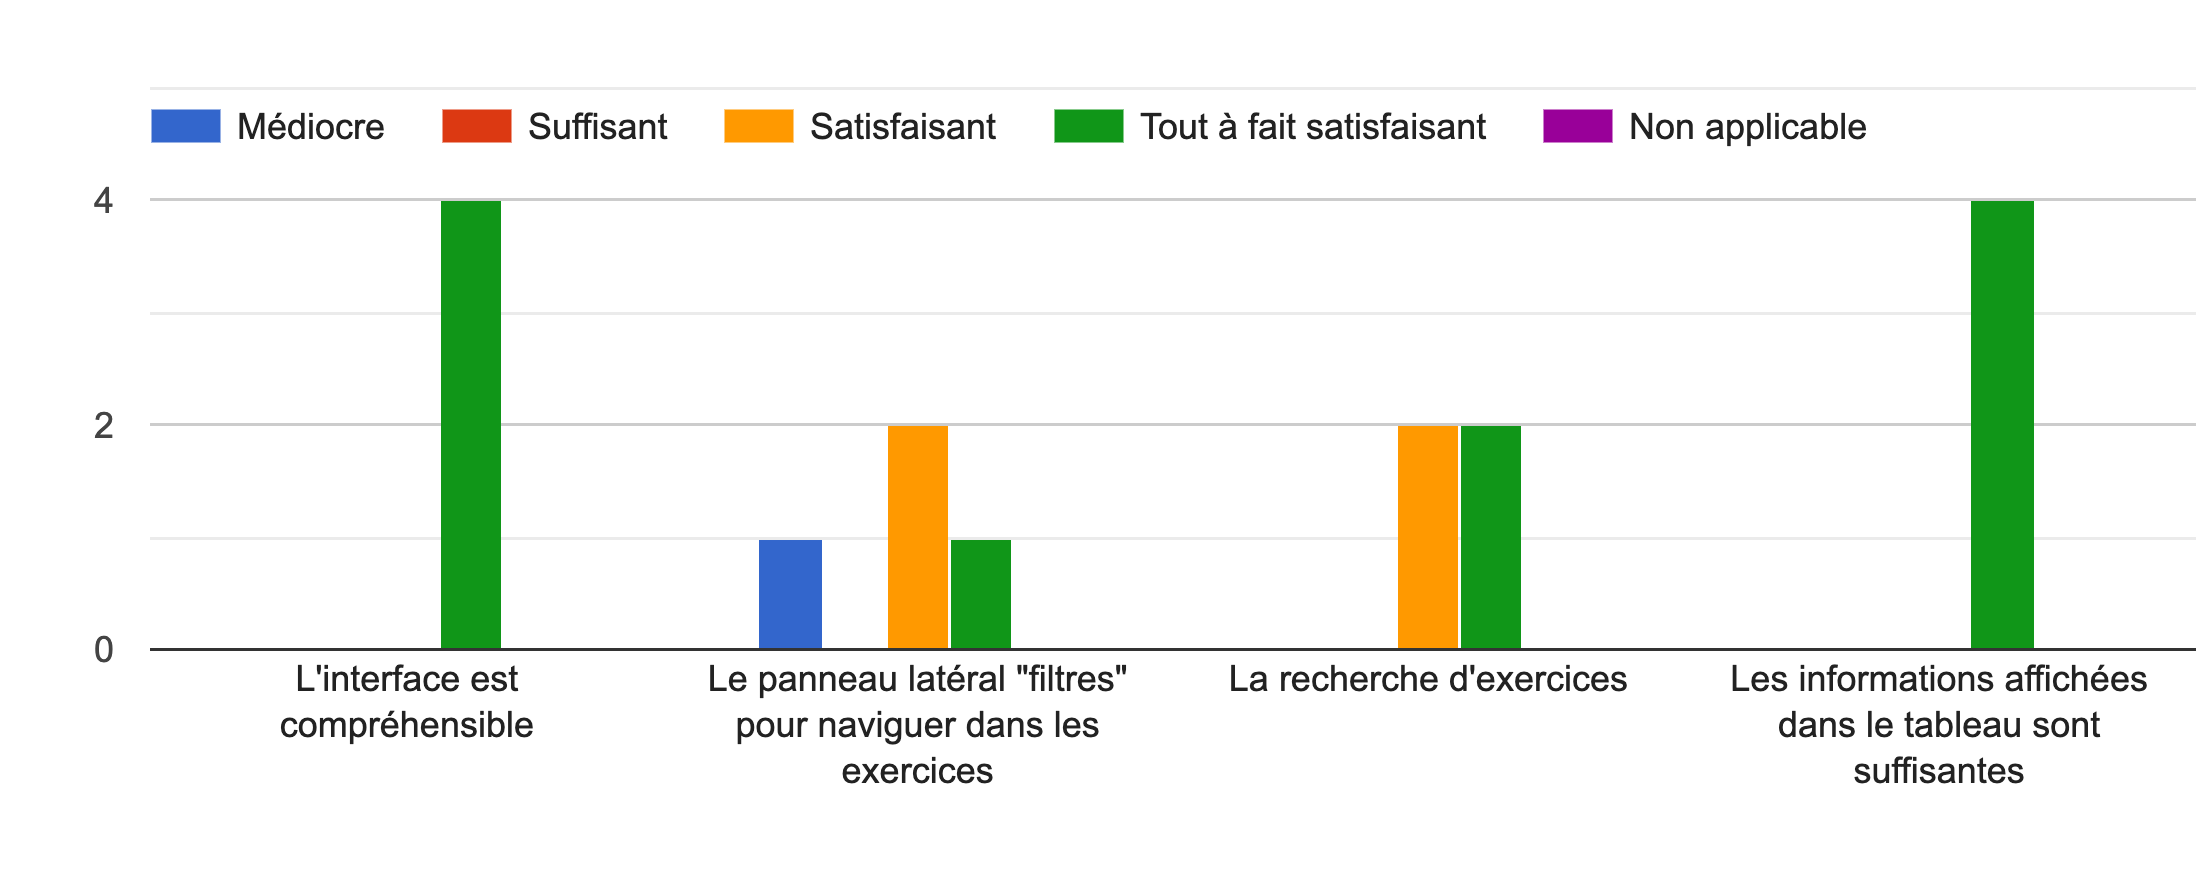
\includegraphics[width=\textwidth,height=0.3\textheight,keepaspectratio]{images/googleForm/gestionResInfo_2.png}
    \centering
\end{figure}

\subsubsection*{Des remarques ?}

\begin{itemize}
    \item Il n'y a actuellement aucune réponse à cette question.
\end{itemize}

\subsubsection*{Page de création/modification d'une ressource informatique}

\begin{figure}[H]
    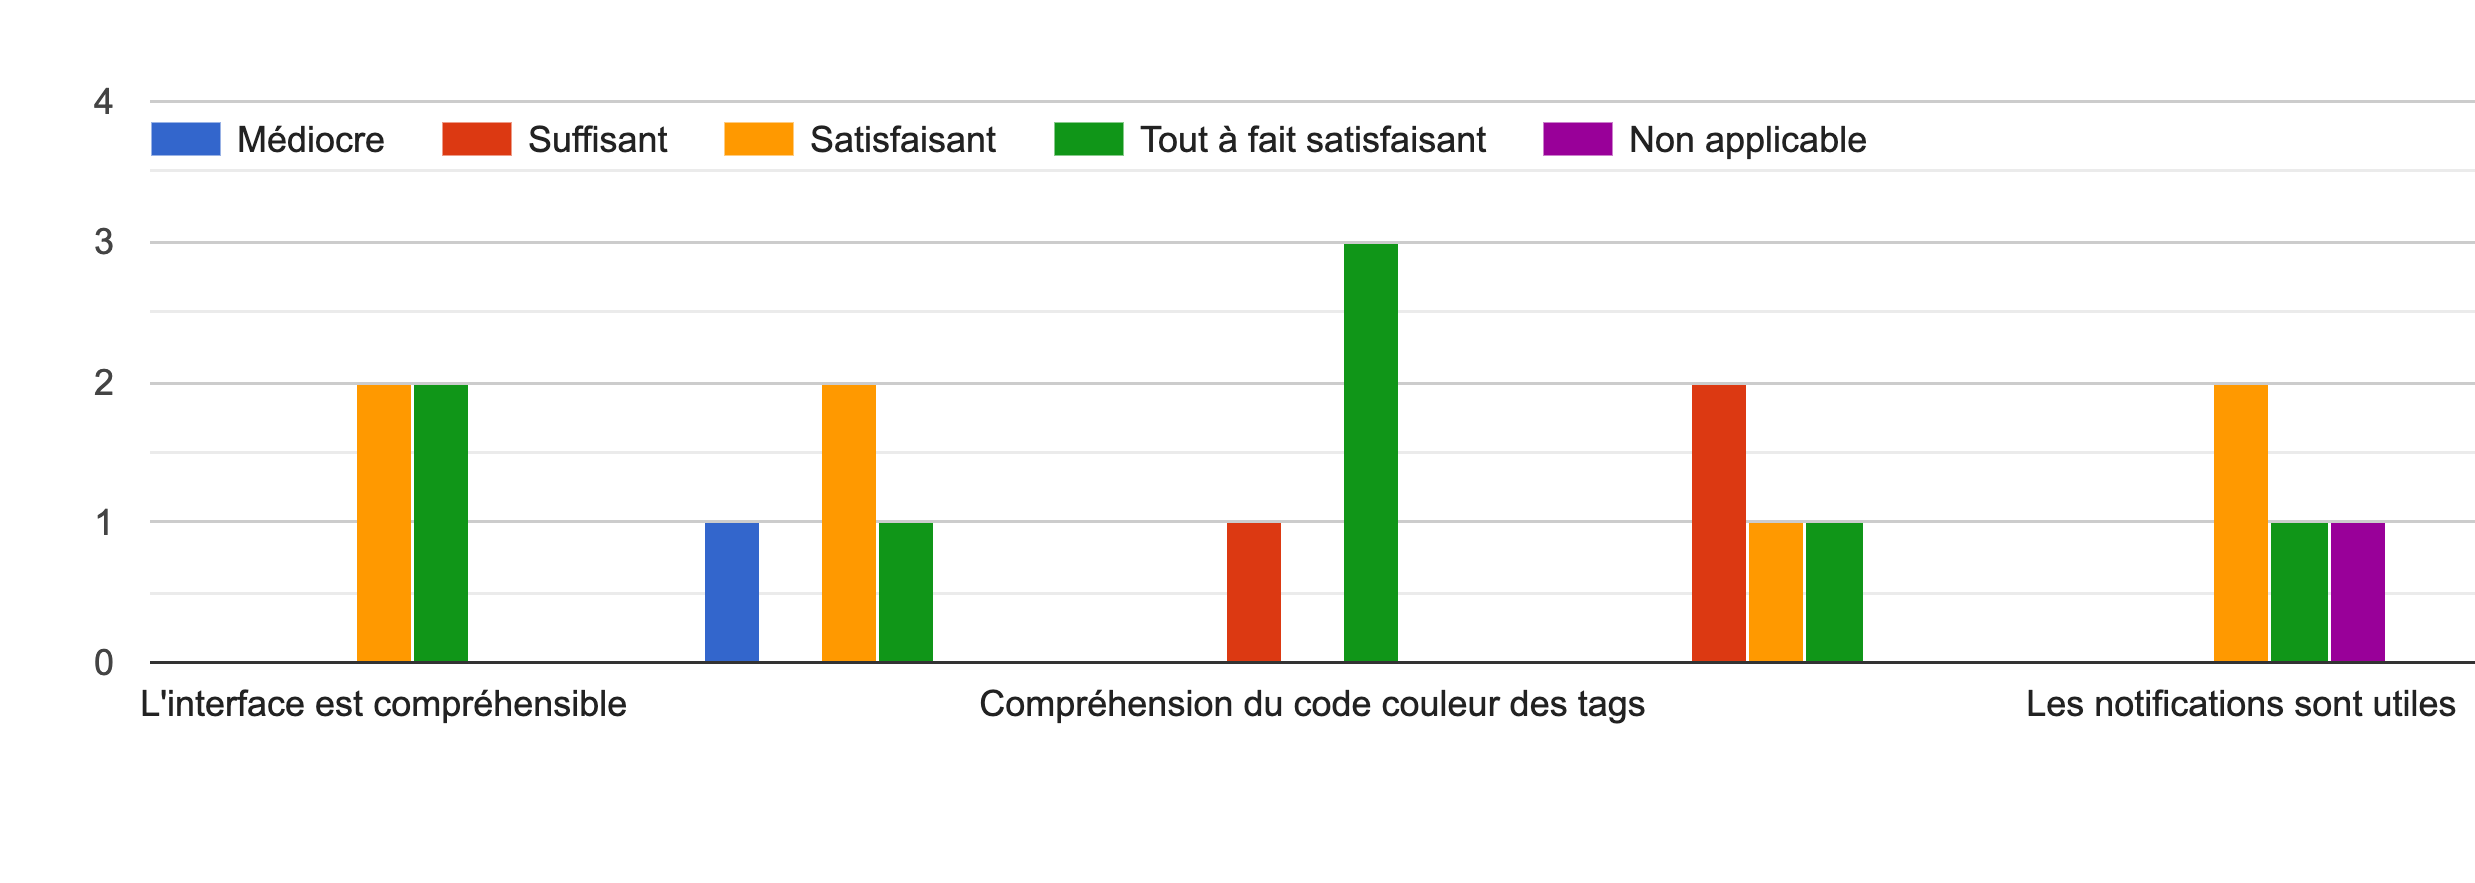
\includegraphics[width=\textwidth,height=0.3\textheight,keepaspectratio]{images/googleForm/creationModifResInfo_2.png}
    \centering
\end{figure}

\subsubsection*{Des remarques ?}

\begin{itemize}
    \item Beaucoup de travail pour la gestion d'un tag
\end{itemize}

\section{Questions ouvertes}

\subsection*{Quels sont les points forts de cette application ?}

\begin{itemize}
    \item Ergonomique et riche en filtres de recherche (utile puisque le but est de rassembler une grande quantité d'exos)
    \item Elle est très complète
    \item Très utile si il y a une grande communauté et qu'il y a beaucoup d'exercice. Et la sélection dynamique est top.
    \item Design visuel, fluidité
    \item Son design, très ergonomique, lisible et claire, bon agencement des composants
    \item L'idée de rassembler toutes les ressources informatiques au même endroit me semble pertinent et utile. En plus, le système de tags (utilisés correctement par vos utilisateurs, ça vous ne pouvez pas garantir) me semble flexible et potentiellement très utile
    \item Application très complète et visuellement attrayante
\end{itemize}

\subsection*{Quels sont les points faibles de cette application ?}

\begin{itemize}
    \item C.f. remarques et détails de la partie précédente
    \item Beaucoup d'information pas toujours facilement identifiable.
    \item Si il n'y a que peu d'exercice, la plateforme aura peu d'intérets. Et il faut aussi voir si les admins ne risquent pas d'etre débordés de requetes en cas de trop grande affluence
    \item Clarité et association visuelle
    \item Le nombre d'actions à faire pour une recherche, de manière générale
    \item Beaucoup de menus et de scroll bars, la learning curve sera donc un peu compliquée pour les utilisateurs les moins "tech savy" (vous seriez surpris du niveau des profs, même d'informatique parfois !)
    \item La gestion des tags m'a semblé un peu lourde et complexe. Beaucoup d'éléments dans les menus sur le côté, ce qui est un point faible au début de la prise en main de l'application mais qui deviendra un point fort après avoir bien pris en main l'application.
\end{itemize}

\subsection*{Quels sont les points faibles de cette application ?}

\begin{itemize}
    \item Il s'agit d'un produit bien abouti ! Je dirais que c'est un stade où c'est une masse d'utilisateurs et de feedback qui permettraient de déterminer les différentes voies d'amélioration.
    (D'ailleurs, tout ce qui a été relevé pendant le call relève davantage du détails et de petites mises à jour que de réels problèmes à fix.)
    \item Clarifier l'interface. L'UI représente cependant beaucoup de travail. Je cois que vous avez priorisé les bonnes choses.
    \item Permettre une vérification par la communauté et par des utilisateurs vérifiés, ou l'ajout d'un tag " non vérifié "
    \item Améliorer l'agencement des menus surtout
    \item Un fonction "mdp oublié" pour les users. Certaines librairies JS font ça assez bien, ça n'est pas spécialement énormément de boulot en plus. Egalement, la possibilité pour ceux qui créent l'exercice d'ajouter une "solution" a l'exercice.
    \item Principalement écouter le feedback des utilisateurs qui font vos validations. Vous êtes bons niveau performances/etc; il manque surtout du polish interface graphique
    \item Gérer cette zone de recherche perdue en haut autrement. C'est ce qui m'a perturbé le plus dans l'utilisation de l'appli.
\end{itemize}

\subsection*{Que manquerait-il pour que cette application ne soit plus un prototype en terme de fonctionnalités ?}

\begin{itemize}
    \item Je ne vous rejoins pas sur l'idée que Source Code en est au stade de "prototype". Ca ressemble bien plus à un produit fini, en une première version, qui peut être concernée par d'éventuelles mises à jour par la suite.
    \item Pas grand chose, et beaucoup à la fois. Il s'agit du lent travail de lisser les bugs et les surprises que peuvent rencontrer les utilisateurs.
    \item peut etre un complétion " automatique " dans la barre de recherche et permettre la recherche de mot clés dans le titre et pas juste tout le titre genre pour trouver les while loops pouvoir taper " loop"
    \item Rien. Pour moi c'est + qu'un prototype au stade où elle en est. Cela dit, s'il fallait vraiment ajouter UNE seule feature, je mettrais celle où, le créateur d'un exercice peut "ajouter une solution" et un autre utilisateur pourrait "proposer une solution" qui serait soumise à approbation de celui qui a créé l'exercice.
    \item Une manière d'interagir entre les étudiants et les "créateurs d'exercices" ? Histoire de pouvoir au moins poser des questions et pas être aussi détachés
    \item Rien
\end{itemize}

\subsection*{Dans une perspective où ce projet ne serait plus un prototype et ne souffrirait plus de ces points faibles : Pensez-vous que cette application ait un réel impact dans le monde des ressources partagées ?}

\begin{itemize}
    \item Oui
    \item Oui, très bonne idée. Il faudrait juste voir comment gérer l'accès entre votre plateforme et celles qui permettent la correction des exos (expl Inginious). Par exemple un moyen de linker votre plateforme avec les autres, pour qu'en un clic on arrive directement sur l'exo inginious en étant déjà connecté dessus.
    \item Sans être intégrée à une plateforme automatisée de correction de code, et sans une gestion de parcours et de lien en tre les exercices, sans doute pas beaucoup. Elle sera limitée à une utilisation par les enseignants pour créer leurs propres cours.
    \item Oui je pense que ca peut être utile
    \item Je ne sais pas, car d'autres plateformes similaires existent et ont la fonctionnalité "ajouter une solution" ou même de "soumettre en ligne".
    \item Oui, cela peut avoir une belle valeur ajoutée.
\end{itemize}

\subsection*{Avez-vous eu recourt à la section tutoriel ?}

\begin{itemize}
    \item Non
    \item Oui pour l'édit de texte
    \item Très sommairement.
    \item Avant de commencer la session de tests, pas après
\end{itemize}

\subsection*{Utiliseriez-vous cette plateforme ? Si oui, quel serait alors votre activité principale ? Si non, pourquoi ?}

\begin{itemize}
    \item Je pense que pour des professeurs, cela peut être très utile pour trouver et donner des exos à des étudiants (ou d'avoir des idées)
    \item Trouver des idées d'exercices pour compléter mes cours.
    \item non, je pense que ça s'appliquerait surtout au domaine éducatif
    \item Oui
    \item Oui, en tant que Professeur / enseignant, pourvu que les solutions soient mises à dispositions.
    \item Sans doute pas, dans la mesure ou INGInious fait des choses similaires tout en étant open source et présent dans tous les environnements auxquels je suis confrontée.
    \item Oui, je pourrais l'utiliser. Recherche d'idées dans divers domaines.
\end{itemize}











